\documentclass[border=10pt]{standalone}
\usepackage[utf8]{inputenc}
\usepackage[T1]{fontenc}
\usepackage{tikz}
\usetikzlibrary{shapes.geometric, arrows.meta, positioning, shadows}

\begin{document}

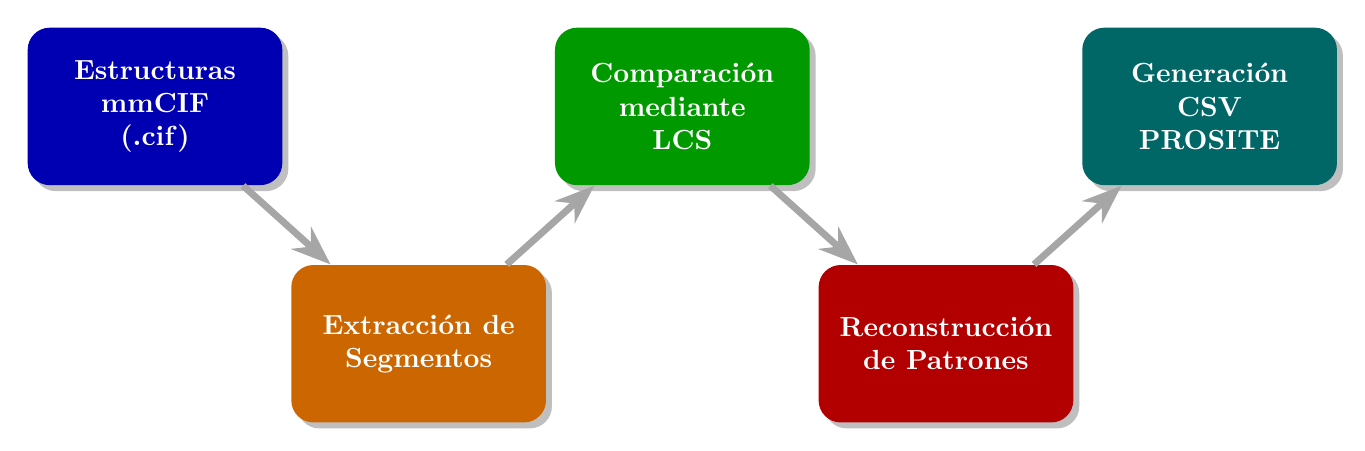
\begin{tikzpicture}[
        node distance=0.8cm and 1cm,
        % Estilos para nodos principales
        mainbox/.style={
                rectangle,
                rounded corners=8pt,
                minimum width=3.2cm,
                minimum height=2cm,
                text centered,
                text width=3cm,
                font=\bfseries\normalsize,
                text=white,
                drop shadow
            },
        % Flechas
        arrow/.style={
                ->,
                >=Stealth,
                line width=2.5pt,
                color=gray!70
            }
    ]

    % ENTRADA (arriba)
    \node[mainbox, fill=blue!70!black] (entrada) {Estructuras\\mmCIF\\(.cif)};

    % EXTRACCIÓN (abajo-derecha)
    \node[mainbox, fill=orange!80!black, below right=1cm and 0.1cm of entrada] (extraccion) {Extracción de\\Segmentos};

    % COMPARACIÓN (arriba-derecha)
    \node[mainbox, fill=green!60!black, above right=1cm and 0.1cm of extraccion] (comparacion) {Comparación\\mediante\\LCS};

    % RECONSTRUCCIÓN (abajo-derecha)
    \node[mainbox, fill=red!70!black, below right=1cm and 0.1cm of comparacion] (reconstruccion) {Reconstrucción\\de Patrones};

    % SALIDA (arriba-derecha)
    \node[mainbox, fill=teal!80!black, above right=1cm and 0.1cm of reconstruccion] (salida) {Generación\\CSV\\PROSITE};

    % FLECHAS
    \draw[arrow] (entrada) -- (extraccion);
    \draw[arrow] (extraccion) -- (comparacion);
    \draw[arrow] (comparacion) -- (reconstruccion);
    \draw[arrow] (reconstruccion) -- (salida);

\end{tikzpicture}

\end{document}
